\section{Realisierung}
\label{sec:realisierung}

Beschreiben die bisherigen Kapitel, wie der Prototyp aufgebaut werden \textit{soll}, geht es in diesem Kapitel darum, was tatsächlich umgesetzt worden \textit{ist}. Der Prototyp basiert auf der Architekturvariante, die in \secref{sec:variante-4-messaging} beschrieben worden ist.

Als Messaging-Lösung kommt RabbitMQ mit dem AMQP-Protokoll zum Einsatz (siehe \secref{sec:wahl-der-message-queue}).

Die Quellcodeartefakte und Modelldaten befinden sich im Abgabeordner (\texttt{Zusatz/}) im Unterverzeichnis \texttt{deepxray/}.

\subsection{Modellkomponenten}

Die bestehenden Machine-Learning-Modelle wurden im Abschnitt \secref{sec:bestehende-modelle} in ihrer Funktionsweise grob beschrieben. Die eigentlichen Modelle werden um weiteren Code ergänzt, wodurch diese mit der Aussenwelt interagieren können. Die Kombination aus den eigentlichen Modellen und dem zusätzlichen Code zur Interaktion mit der Aussenwelt ‒ der \textit{Integrationscode} ‒ wird als \textit{Modellkomponente} bezeichnet. Für Komponente und Modell werden die gleichen Bezeichnungen verwendet; ob das Modell oder die Modellkomponente gemeint ist, ergibt sich dabei aus dem Kontext. Sämtliche Modellkomponenten sind in Python geschrieben (siehe \secref{sec:wahl-der-programmiersprache-modellkomponenten}).

Die Modellkomponenten wurden alle nach dem gleichen Schema aufgebaut, wobei die Extraktion der Gelenke (\texttt{joint\_detection}) aufgrund der zehn verschiedenen Modelle etwas aus der Reihe tanzt.

Für jede Modellkomponente gibt es eine \textit{Hauptklasse}, die den jeweiligen Einstiegspunkt (Hauptprogramm) für die Komponente darstellt. Dazu kommt eine \textit{Predictor}-Klasse, die das Machine-Learning-Modell kapselt und ein Interface für dieses anbietet. Die Hauptklasse kümmert sich um die Kommunikation mit der Message-Queue. Eingehende Nachrichten werden für den Predictor aufbereitet. Es folgt der Aufruf des Predictors, der das Ergebnis an die Hauptklasse zurückliefert. Hier wird die Antwort interpretiert (Erfolg oder Fehler) und an die entsprechende Message-Queue weitergeleitet.

Innerhalb der Modellkomponenten erfolgt die Abarbeitung synchron: Von der eingehenden Queue wird jeweils nur eine Message geholt und verarbeitet. Erst dann wird die nächste Message entgegengenommen und wiederum verarbeitet. Die parallele Verarbeitung erfordert somit, dass mehrere Instanzen pro Modellkomponente am Laufen sind.

\subsubsection{Aufbau der Modellkomponenten}
\label{sec:aufbau-der-modellkomponenten}

Diese verallgemeinerte Struktur wird im Klassendiagramm auf \imgref{fig:klassendiagramm-generisch} veranschaulicht. Die Hauptklasse (\texttt{Main}) verfügt jeweils über eine Verbindung mit dem Message-Broker (\texttt{connection}) und einen Kanal (\texttt{channel}), der über diese Verbindung kommuniziert. Eine \texttt{Predictor}-Instanz wird im Konstruktor der \texttt{Main}-Klasse erzeugt. Im Konstruktor (\texttt{\_\_init\_\_()}) der \texttt{Predictor}-Klasse wird das eigentliche Modell geladen. Hierzu wird ein Modellpfad benötigt, den die \texttt{Main}-Klasse aus einer Umgebungsvariablen liest.

\begin{figure}[tbh]
    \centering
    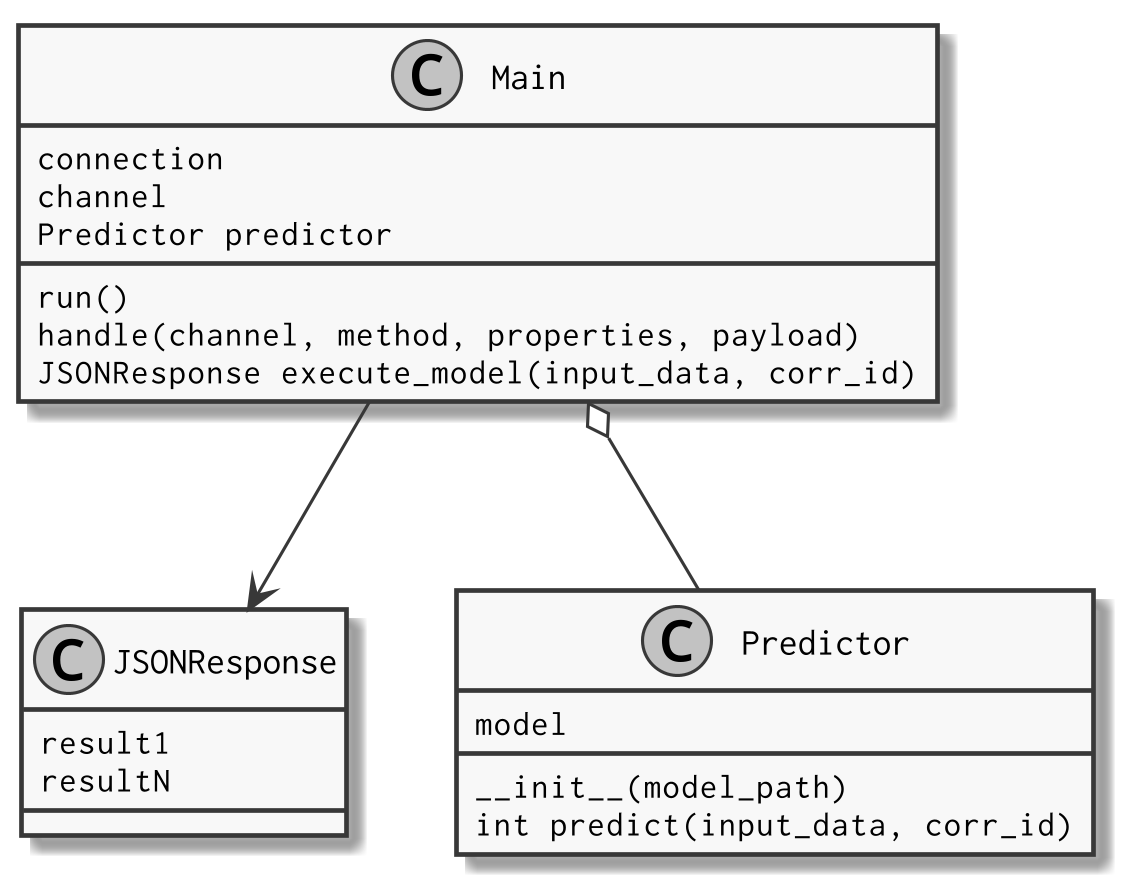
\includegraphics[width=0.9\linewidth]{pics/class-generic.png}
    \caption{Die allgemeine Architektur der Modellkomponenten, bestehend aus einer Hauptklasse und einer Predictor-Klasse. (Klassendiagramm)}
    \label{fig:klassendiagramm-generisch}
\end{figure}

Die \texttt{run()}-Methode wird vom Hauptprogramm aufgerufen, sobald die Klasse instanziiert ist. Diese stellt sicher, dass alle benötigten Queues vorhanden sind, registriert die Callback-Methode für eingehende Nachrichten (\texttt{handle()}), und lässt anschliessend auf eingehende Nachrichten warten.

Die \texttt{handle()}-Methode wird automatisch aufgerufen, sobald eine Nachricht aus der Queue eintrifft. Diese hat per API-Definition vier Parameter: Der \texttt{channel} wird dazu benötigt, um Nachrichten aus dem Callback heraus zu publizieren (etwa um Antworten zu senden). Der Parameter \texttt{method} ist ein AMQP-Delivery-Object, welches hier dazu dient, die Verarbeitung der Nachricht zu bestätigen, um darauf die nächste Nachricht zu erhalten. Der \texttt{properties}-Parameter enthält verschiedene Informationen, wovon hier nur der Correlation Identifier (\texttt{corr\_id}) relevant ist. Dieser wird benötigt, um ausgehende Nachrichten dem gleichen Vorgang zuzuordnen wie die eingegangene Nachricht.\footnote{Das Konzept des Correlation Identifiers wird in Abschnitt \secref{sec:variante-3-messaging} erklärt.} Der \texttt{body}-Parameter schliesslich enthält den Payload der Nachricht, sprich die eigentlichen Nutzdaten.

Beim Payload handelt es sich meistens um eine JSON-Datenstruktur. Diese enthält ein Bild (ganzes Röntgenbild oder nur einen einzelnen Gelenkausschnitt davon) und im Falle der Extraktion und des Scorings noch eine Gelenkbezeichnung. Das Bild ist jeweils als base64-kodierte Zeichenkette abgelegt.\footnote{Dieses Austauschformat wurde aufgrund früherer positiver Erfahrung in verschiedenen Projekten gewählt, ohne dass hierzu ausführlich Alternativen geprüft worden sind. \textit{Protocol Buffers} dürften aufgrund des binären Übertragungsformats eine höhere Effizienz ermöglichen, jedoch auch eine höhere Komplexität ‒ eine zusätzliche Notation und einen weiteren Build-Schritt ‒ mit sich bringen \cite{protobuf}. Zudem erschien es dem Autor dieser Arbeit vernünftiger, die Anzahl der für ihn neuen Technologien und Konzepte ‒ Machine Learning, Messaging via AMQP ‒ innerhalb eines Projekts nicht weiter auszudehnen. Die Codierung, Übertragung und Dekodierung der Bilder stellt auch bei Weitem nicht den Flaschenhals in der Verarbeitung dar, wodurch der Einsatz von Protocol Buffers wohl kaum spürbare Performanceauswirkungen auf das Gesamtsystem hätte.} Das Bild wird dekodiert und ‒ wenn nötig mit Zusatzinformationen; zwecks Logging immer mit dem Correlation Identifier (\texttt{corr\_id})  ‒ an die \texttt{execute\_model()}-Methode übergeben. Diese kapselt den Aufruf der \texttt{predict()}-Methode der \texttt{Pre\-dictor}-Instanz.

Die \texttt{predict()}-Methode führt die Prediction auf Basis des Modells aus, wovor teilweise noch einzelne Verarbeitungsschritte zu erfolgen haben (\textit{Preprocessing}). Die ermittelte Prediction (der Output des Modells) wird von der Methode zurückgeliefert. Dieser wird von der \texttt{execute\_model()}-Methode in eine JSON-Struktur (im Klassendiagramm als \texttt{JSONRe\-sponse} bezeichnet\footnote{Diese Klasse ist rein konzeptionell zu verstehen. Tatsächlich findet sich in keiner der drei Modellkomponenten eine Python-Klasse dieses Namens. Es handelt sich vielmehr jeweils um ein Dictionary (\texttt{dict}), das die aufgelisteten Eigenschaften enthält. Eine Implementierung in Java würde hier tendenziell eine Klasse verwenden, bei Go dürfte eine Struktur zum Einsatz kommen.}) verpackt und an die \texttt{handle()}-Methode zurückgegeben, welche diese wiederum als Payload an die Ergebnis-Queue weitergibt. Tritt in diesem Prozess ein Fehler auf, wird von \texttt{predict()} eine entsprechender Exception geworfen, der erst von \texttt{handle()} abgefangen und als Fehlermeldung an die Fehler-Queue weitergereicht wird.

Dieser Prozess beschreibt die Arbeitsweise der Modellkomponenten im Allgemeinen. In den folgenden Abschnitten für die einzelnen Modellkomponenten wird nur noch auf Erweiterungen und Abweichungen dieses allgemeinen Schemas eingegangen. Auf weitere gemeinsame Aspekte, die eher technischer Natur sind, wird im Abschnitt \secref{sec:gemeinsame-technische-aspekte} eingegangen, der als Anhang zu diesem Unterkapitel zu lesen ist.

\subsubsection{Modellkomponente \texttt{body\_part}}
\label{sec:modellkomponente-body-part}

Das Erkennen eines Körperteils ist der erste Schritt in der Verarbeitung eines Röntgenbildes, bei dem ein Machine-Learning-Modell zum Einsatz kommt. Das Klassendiagramm dieser Komponente (siehe \imgref{fig:klassendiagramm-body-part}) entspricht dabei weitgehend demjenigen der generischen Modellkomponente.

\begin{figure}[tbh]
    \centering
    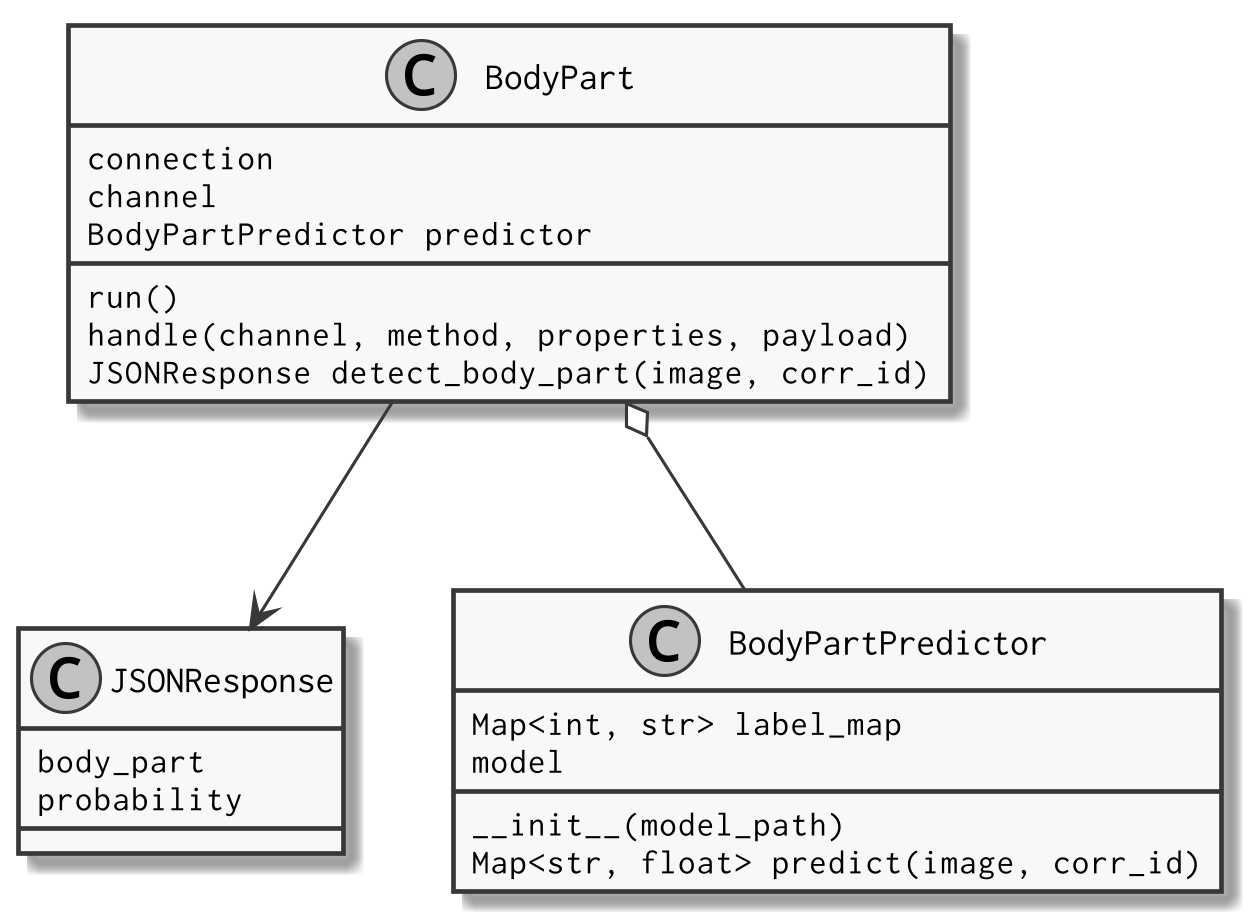
\includegraphics[width=0.9\linewidth]{pics/class-body-part.png}
    \caption{Die Modellkomponente \texttt{body\_part} entspricht in ihrer Klassenstruktur weitgehend der generischen Modellkomponente. (Klassendiagramm)}
    \label{fig:klassendiagramm-body-part}
\end{figure}

Die Unterschiede zur generischen Komponente liegen bei Input und Output von \texttt{body\_part}. Auf einem Röntgenbild (Input) wird erkannt, um welches Körperteil es sich mit welcher Wahrscheinlichkeit handelt. Die Körperteile werden mithilfe der \texttt{label\_map} in \texttt{BodyPartPredictor} zu den numerischen Outputs gemappt (das Label \texttt{hand left} hat den Output 6). Die \texttt{predict()}-Methode gibt eine Map von Körperteilen mit Wahrscheinlichkeiten zurück. In \texttt{detect\_body\_part()} wird dann das Körperteil mit der höchsten erzielten Wahrscheinlichkeit ausgewählt. Körperteil und Wahrscheinlichkeit werden zurückgegeben, damit letztere gegen eine vordefinierte Schwelle (z.B. mindestens 50\% Wahrscheinlichkeit) geprüft werden könnte.

Beide Informationen ‒ erkanntes Körperteil und Wahrscheinlichkeit ‒ werden mit der \texttt{JSONResponse} an den Client zurückgeliefert, damit dieser eine allfällige Schwellenwertprüfung selber durchführen könnte.

Die \texttt{run()}-Methode der \texttt{BodyPart}-Klasse konsumiert Nachrichten von einer Queue namens \texttt{body\_part}. Als Payload werden rohe JPEG-Daten (eine Reihe von Bytes) erwartet; eine Einbettung in JSON mit base64-Kodierung entfällt hier. Resultate werden auf einer Queue namens \texttt{body\_part\_response} publiziert.

Die Klasse \texttt{BodyPartPredictor} wird mit dem Integrationstest (\texttt{test\_body\_part\_pre\-dic\-tor.py}) im \texttt{tests/}-Unterverzeichnis getestet. Dieser prüft für verschiedene Röntgenbilder einer linken Hand, ob diese korrekt als das wahrscheinlichste Körperteil erkannt wird, und dass die Wahrscheinlichkeit in einem Bereich zwischen 0 und 1 liegt (Plausibilität). Für eine Röntgenaufnahme eines linken Fusses wird geprüft, dass auf dem Bild \textit{nicht} eine linke Hand erkannt wird.

\subsubsection{Modellkomponente \texttt{joint\_detection}}

Die Extraktion der Gelenke ist der aufwändigste Arbeitsschritt in der Verarbeitung von Röntgenbildern. Für jedes der zehn relevanten Gelenke (MCP 1-5, PIP 1-5) wird ein separates Modell benötigt. Eine \texttt{Predictor}-Klasse, die ein Modell lädt und verwendet, genügt bei der Modellkomponente \texttt{joint\_detection} nicht den Anforderungen.

Die einzelnen Modelle werden daher nicht über die \texttt{Predictor}-Klasse (\texttt{JointDetection\-Predictor}) abstrahiert, sondern über eine gesonderte \texttt{Model}-Klasse namens \texttt{Joint\-De\-tec\-tion\-Model}. Die \texttt{Predictor}-Klasse verfügt intern über eine Datentstruktur (ein Dictionary namens \texttt{models}), die eine Gelenkbezeichnung (\texttt{pip1}, \texttt{mcp3} usw.) einer Instanz von \texttt{Joint\-De\-tectionModel} zuordnet. Für die eigentliche Prediction wird in der \texttt{predict()}-Methode von \texttt{Joint\-De\-tec\-tion\-Predictor} anhand des Gelenknamens die entsprechende \texttt{Model}-Klas\-se aus dem \texttt{models}-Dictionary gelesen, worauf anschliessend die \texttt{predict()}-Methode der jeweiligen \texttt{Joint\-De\-tec\-tion\-Model}-Klasse mit dem Röntgenbild aufgerufen werden kann. (Der Gelenkname ist durch den Kontext gegeben und wird über den Konstruktor festgelegt.) Diese Klassenstruktur ist auf \imgref{fig:klassendiagramm-joint-detection} zu sehen.

\begin{figure}[H]
    \centering
    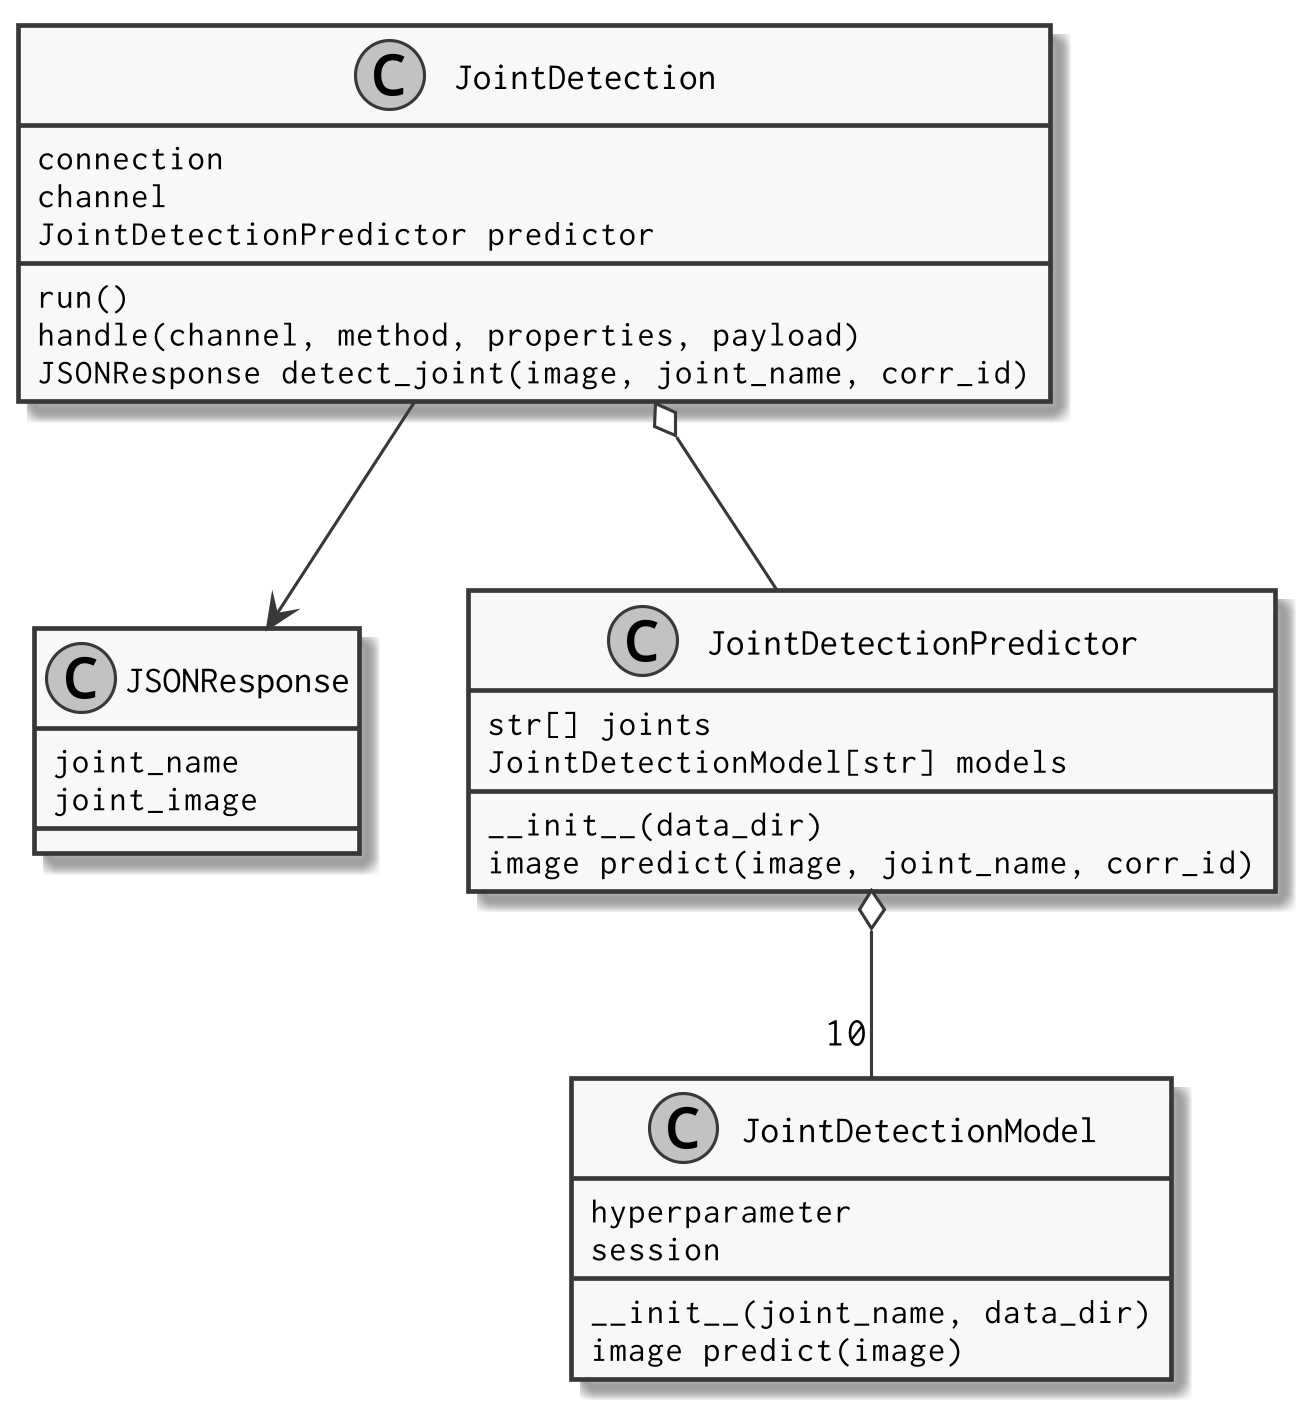
\includegraphics[width=0.9\linewidth]{pics/class-joint-detection.png}
    \caption{Die Modellkomponente \texttt{joint\_detection} verwendet zehn verschiedene Modelle und abstrahiert diese über eine zusätzliche Klasse namens \texttt{Joint\-Detection\-Model}. (Klassendiagramm)}
    \label{fig:klassendiagramm-joint-detection}
\end{figure}

Die Modellkomponente \texttt{joint\_detection} wird nicht nur einmal für alle zehn Gelenke aufgerufen (bzw. über eine entsprechende Message über die Queue \texttt{joint\_detection} angestossen), sondern einmal pro Gelenk (siehe \secref{sec:variante-4-messaging}). Darum dient als Input nicht nur ein Röntgenbild, sondern auch die Bezeichnung des zu extrahierende Gelenks. Der Payload ist eine JSON-Datenstruktur, die somit aus den Feldern \texttt{joint\_name} (Zeichenkette der Länge 4) und \texttt{xray} (base64-kodiertes JPEG-Bild) besteht.

Der Output des Modells ist wiederum ein JPEG-Bild, das base64-kodiert in der \texttt{JSONRe\-sponse} im Feld \texttt{joint\_image} abgelegt wird. Der Name des Gelenks (Feld \texttt{joint\_name}) wird auch in diese Datenstruktur eingebettet, da diese Information im nächsten Verarbeitungsschritt benötigt wird. So wird das Ergebnis nicht an den Aufrufer zurückgeliefert, sondern an die Queue \texttt{ratingen\_score} weitergeschickt. Allfällige Fehler werden in die Queue \texttt{joint\_detection\_error} geschrieben (JSON-Datenstruktur mit den Feldern \texttt{error} für die Fehlermeldung und \texttt{joint\_name} für die Gelenkbezeichnung).

Die Gelenkbezeichnung muss in jedem Fall ‒ Fehler oder Erfolg ‒ weitergegeben werden, da der \texttt{orchestrator} seinen Client erst bedienen kann, wenn er für jedes Gelenk eine Nachricht erhalten hat (siehe \secref{sec:variante-4-messaging}).

Die Klasse \texttt{JointDetectionPredictor} wird mit dem Integrationstest (\texttt{test\_joint\_de\-tect\-ion\_predictor.py}) im \texttt{tests/}-Unterverzeichnis getestet, der alle zehn Modelle für verschiedene Röntgenbilder ausführt, und prüft, ob jeweils ein Bildausschnitt zurückgeliefert wird.

\subsubsection{Modellkomponente \texttt{ratingen\_score}}

Das Scoring der Gelenke erfordert wiederum nur die Ausführung eines einzigen Machine-Learning-Modells, das mit allen zehn Gelenken gleichermassen umgehen kann. Der Parameter \texttt{joint\_name} ist für die eigentliche Prediction irrelevant, wird aber zwecks Logging trotzdem durch verschiedene Methoden gereicht. Auch im Scoring-Ergebnis (\texttt{JSON\-Re\-sponse}) muss das Gelenk vermerkt sein, damit der \texttt{orchestrator} das betreffende Gelenk beim Eintreffen der Message für den jeweiligen Vorgang als erledigt markieren kann. Die Klassesnstruktur ist auf \imgref{fig:klassendiagramm-ratingen-score} zu sehen.

\begin{figure}[tbh]
    \centering
    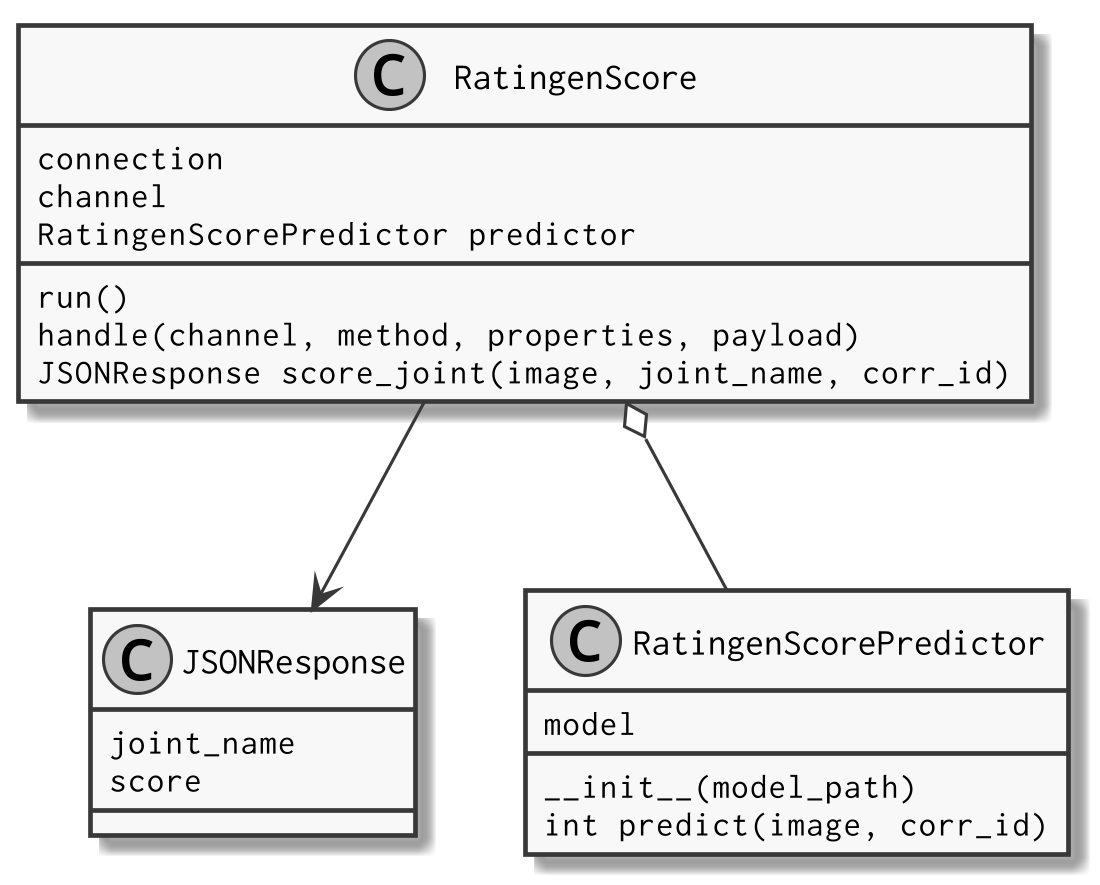
\includegraphics[width=0.9\linewidth]{pics/class-ratingen-score.png}
    \caption{Die Modellkomponente \texttt{ratingen\_score} entspricht (ähnlich wie \texttt{body\_part} in ihrer Klassenstruktur weitgehend der generischen Modellkomponente. (Klassendiagramm)}
    \label{fig:klassendiagramm-ratingen-score}
\end{figure}

Das Modell hinter dem \texttt{RatingenScorePredictor} erwartet das Bild eines Gelenks im JPEG-Format als Input, das im JSON-Payload über das Feld \texttt{joint\_image} base64-kodiert mitgegeben wird. (Das Feld \texttt{joint\_name} im JSON-Payload bezeichnet das Gelenk.) Der Output des Modells ist eine Score im Wertebereich von 0 bis 5 (siehe \secref{sec:modell-ratingen-score} zur Bedeutung dieser Scores).

Die Inputs werden von der Queue \texttt{ratingen\_score} gelesen, die Ergebnisse auf die Queue \texttt{scores} (im Erfolgsfall, mit Gelenkname und Score) bzw. \texttt{ratingen\_score\_error} (im Fehlerfall, mit Gelenkname und Fehlermeldung) geschrieben.

Die Klasse \texttt{RatingenScorePredictor} wird mit dem Integrationstest (\texttt{test\_ratingen\_score\_predictor.py}) im \texttt{tests/}-Unterverzeichnis getestet, der zehn zuvor eigenhändig ausgeschnittene Bilder von Gelenken einem Scoring unterzieht, und das Ergebnis auf Plausibilität (Wertebereich 0 bis 5) prüft.

\subsubsection{Gemeinsame technische Aspekte}
\label{sec:gemeinsame-technische-aspekte}

Die strukturellen Gemeinsamkeiten der drei Modellkomponenten wurden im Abschnitt \secref{sec:aufbau-der-modellkomponenten}  erörtert. Hier soll es nachgelagert um die \textit{technischen} Gemeinsamkeiten der erörterten Modellkomponenten gehen. Dies sind:

\begin{description}
    \item[Container] Die Modellkomponenten werden in Docker-Containern ausgeführt (siehe \secref{sec:austauschbarkeit-von-modellen}). Die Images, die jeweils im \texttt{Dockerfile} der jeweiligen Modellkomponente definiert sind, unterscheiden sich dabei voneinander. Dies hat einerseits mit den unterschiedlichen Python-Versionen (siehe \secref{sec:wahl-der-programmiersprache-modellkomponenten}), andererseits mit den komponentenspezifischen Details (Modelldaten, Abhängigkeiten der verwendeten Libraries/Frameworks in \texttt{requirements.txt} und der Code-Struktur) zu tun. Gemeinsam haben alle Images, dass sie auf einem offiziellen Python-Image basieren, die Modelldaten und den Quellcode in zwei verschiedene Verzeichnisse kopieren, alle Abhängigkeiten automatisch aus der Datei \texttt{requirements.txt} installieren, und die Hauptklasse des jeweiligen Modells ausführen.
    \item[Testing] Die verschiedenen Testfälle (Integrationstests) wurden bereits im Kontext jeder Modellkomponente kurz erläutert. Da sich die Modelle nur in einem Container ausführen lassen, müssen auch die Tests in einem Container laufen. Hierzu wird jeweils im \texttt{tests/}-Unterverzeichnis jeder Modellkomponente ein weiteres Image definiert, das auf dem Image der Modellkomponente basiert. Für dieses Image wird jeweils das Testing-Framework \texttt{pytest} installiert, der Testcode in den Container kopiert und anschliessend mit \texttt{pytest} ausgeführt. Das Erstellen des Images und Ausführen des Testcontainers erfolgt am einfachsten mit dem Shell-Skript \texttt{test.sh}, das sich im jeweiligen \texttt{tests/}-Verzeichnis befindet.
    \item[Logging] Alle Modellkomponenten geben Log-Meldungen aus. Diese enthalten jeweils den Correlation Identifier am Ende jeder Logzeile in eckigen Klammern. Es wird auf dem Level \texttt{Debug} (Meldungen zum aktuellen Verarbeitungsschritt) und \texttt{Error} (Fehlermeldungen) geloggt. Als Ausgabe dient \texttt{stdout}, und nicht wie üblich \texttt{stderr}, da bei der Ausführung mit \texttt{docker-compose} standardmässig nur Meldungen von der Standardausgabe angezeigt werden. Der Python-Interpreter wird jeweils mit dem Flag \texttt{-u} (unbuffered) gestartet, sodass Log-Meldungen unverzüglich ausgegeben und nicht in einem Puffer zwischengespeichert werden. Auch die Art der Log-Meldungen ist bei allen Modellkomponenten ähnlich, so werden folgende Ereignisse geloggt: Verbindung mit dem Message-Broker (Erfolg/Misserfolg nach \texttt{n} Versuchen), Laden des Modells (mit der dazu benötigten Zeit), Eintreffen eines Payloads (mit dessen Grösse), abgeschlossene Prediction (mit Ergebnis und dazu benötigter Zeit); und allfällige Exceptions (als Fehler). Jede Log-Meldung enthält weiter den genauen Zeitpunkt, das Log-Level und den Namen der Klasse, welche die Log-Meldung ausgegeben hat.
    \item[Verbindungsaufbau] Die Modellkomponenten sind erst voll einsatzfähig, wenn der von ihnen verwendete Message-Broker (RabbitMQ) aufgestartet ist, und sie sich mit diesem verbunden haben. Die Modellkomponenten sind somit vom Message-Broker abhängig, und ihre Container sollten idealerweise erst dann aufgestartet werden, wenn RabbitMQ bereit ist. Leider verfügt \texttt{docker-compose} über keinen Mechanismus, der diese Abhängigkeit zuverlässig abbilden könnte.\footnote{Mit \texttt{depends\_on} kann höchstens geprüft werden, ob ein Container bereits \textit{gestartet} worden ist, und nicht, ob die Container-Anwendung bereits fertig geladen und so etwa für eingehende Verbindungen \textit{bereit} ist.} Aus diesem Grund kann eine Modellkomponente nicht wissen, ob RabbitMQ schon bereit für eingehende Verbindungen ist. Eine einfache Lösung ist der wiederholte Versuch eines Verbindungsaufbaus mit einem \textit{Backoff}, wobei nach jedem gescheiterten Versuch ein bestimmtes Zeitfenster abgewartet wird, bevor ein neuer Verbindungsaufbau versucht wird. Diese Versuche werden in einem Takt von zwei Sekunden unternommen, insgesamt maximal 60 mal. Kann während dieser Zeit keine Verbindung hergestellt werden, dürfte ein Fehler im Gesamtsystem vorliegen, der vor weiteren Verbindungsversuchen zu beheben wäre.
    \item[Gemeinsamer Code] Obwohl die drei Modellkomponenten über gemeinsame Funktionalität verfügen (Verbindungsaufbau, Logging), wird zwischen ihnen keinerlei Code (zumindest kein selbstgeschriebener) geteilt. Stattdessen wurden die beiden Dateien \texttt{amqp.py} und \texttt{log.py} (zusammen ca. 50 Zeilen) für die Modellkomponenten jeweils kopiert und wenn nötig angepasst.\footnote{In \texttt{ratingen\_score} können aufgrund der Python-Version 3.5 keine f-Strings verwendet werden.} Dies mag zunächst nach einer schlechten Praxis und einem \textit{Code Smell} klingen, dürfte aber der einzige Weg sein, die \textit{unabhängige} Weiterentwicklung der Modellkomponenten zu ermöglichen. Basierten die Modellkomponenten auf einer gemeinsamen, selbstgeschriebenen Library (für Logging und Verbindungsaufbau), müsste diese für spezielle Anforderungen der Modellkomponenten jeweils angepasst und/oder erweitert werden, was die Vorwärtskompatibilität zu den anderen Modellkomponenten einschränken könnte. Zudem könnten künftige Versionen der Modellkomponenten in einer anderen Programmiersprache als Python geschrieben werden, wodurch die vormals gemeinsame Library nur noch unnötiger Ballast wäre.\footnote{Das Go-Proverb \textit{«A little copying is better than a little dependency.»} bringt zum Ausdruck, dass die Wiederverwendung von Code in manchen Fällen nicht erstrebenswert, ja gar schädlich ist \cite[9:28]{go-proverbs}.}
    \item[Legacy-Code] Die Modellkomponenten \texttt{body\_part} und \texttt{joint\_detection} ‒ sprich die beiden älteren Modelle ‒ enthalten ein \texttt{legacy/}-Verzeichnis. Dieses enthält älteren Code, der grösstenteils ohne Änderung und Reflexion von den Vorprojekten übernommen worden ist. Der Code ist funktionstüchtig, dürfte aber für die Aktualisierung der Modelle auf neuere Frameworks grössere Anpassungen erfordern, und wird im Rahmen der vorliegenden Arbeit nicht analysiert oder dokumentiert.
    \item[Modelldaten] Die Modelldaten werden beim Erstellen des Docker-Images jeweils in dieses hineinkopiert\footnote{Das Einhängen (via \texttt{mount}) über ein lokales Verzeichnis wäre schneller, würde aber die Manipulation der Modelle zur Laufzeit ermöglichen, und bietet daher eine schlechtere Isolation.}, genauer in das Verzeichnis \texttt{/usr/modeldata}.\footnote{Beim Modell \texttt{ratingen\_score} wird zusätzlich das generische Modell \textit{Inception V3} nach \texttt{/root/.keras/models} kopiert, damit die Datei nicht beim Aufstarten des Containers vom Internet heruntergeladen wird, siehe \url{https://stackoverflow.com/q/60837438/6763074} (abgerufen am 23.05.2020).} Das Verzeichnis \texttt{/usr/modeldata} wird der Python-Anwendung via Umgebungsvariable \texttt{DATADIR} zugänglich gemacht, womit die Modelldaten in die Anwendung geladen werden können.\footnote{Bei \texttt{joint\_detection} wird der Pfad zu den Modelldaten zusätzlich über den jeweiligen Gelenknamen ergänzt.}
\end{description}

\subsection{Komponente \texttt{orchestrator}}

Beim \texttt{orchestrator} handelt es sich um die zentrale Komponente des Prototyps. Der Prozess beginnt damit, dass ein Client ein Röntgenbild per HTTP an den \texttt{/score}-Endpoint (\texttt{POST}-Anfrage) sendet, der vom \texttt{orchestrator} angeboten wird, und endet damit, dass der \texttt{orchestrator} dem Client eine Reihe von Scores zurückliefert, idealerweise zehn an der Zahl. Dieser Vorgang ist in \secref{sec:variante-4-messaging} beschrieben und auf \imgref{fig:datenfluss-variante-queue-2} grafisch dargestellt.

Dieser Vorgang dauert einige Sekunden. Währenddessen sollen auch andere Clients Röntgenbilder zur Verarbeitung in Auftrag geben können, ohne auf das Ende eines laufenden Vorgangs warten zu müssen.\footnote{In der Praxis verzögern sich die einzelnen Vorgänge unter starker Last des Systems. Dieses soll aber trotzdem \textit{ansprechbar} bleiben, d.h. die Anfragen zumindest entgegennehmen und in die entsprechenden Queues zur Verarbeitung stellen.} Noch wichtiger ist, dass die Ergebnisse der beiden Vorgänge nicht durcheinandergebracht werden, sodass etwa Anfrager A, der das Röntgenbild einer gesunden Hand verarbeiten lässt, plötzlich die Score für ein geschädigtes Gelenk, das zu einem Bild von Anfrager B gehört, in seinem Ergebnis vorfinden würde.

Wie die nebenläufige Verarbeitung von Röntgenbildern korrekt und möglichst performant erfolgt, wird in Abschnitt \secref{sec:der-score-endpoint} erörtert. Zunächst soll hier aber ein Überblick über die \texttt{orchestrator}-Komponente geboten werden, der zum Verständnis des \texttt{/score}-Endpoints nötig ist.

Der \texttt{orchestrator} ist in Go (siehe \secref{sec:wahl-der-programmiersprache-orchestrator}) geschrieben, genauer in der derzeit aktuellen Version 1.14 von Go. Das \texttt{orchestrator/}-Ver\-zeich\-nis enthält die folgenden Artefakte:

\begin{description}
    \item[\texttt{Dockerfile}] Wie die Modellkomponenten läuft auch der \texttt{orchestrator} in einem Docker-Container. Aufgrund der kompilierten Natur von Go empfiehlt sich hier der Einsatz zwei verschiedener Container: einer für die Kompilierung, und einer für die Ausführung.\footnote{Im Gegensatz zu Python, das einen Interpreter zur Ausführung benötigt, kommen kompilierte Go-Programme gänzlich ohne Laufzeitumgebung aus, da die statisch gelinkten Binärdateien sämtliche Abhängigkeiten beinhalten.} Das \textit{Builder}-Image basiert auf einer aktuellen Version des Go-Docker-Images. Sämtliche Quellcodedateien, sowie die Moduldateien (\texttt{go.mod} und \texttt{go.sum}, siehe weiter unten), werden in das Image kopiert. Die Abhängigkeiten werden mit \texttt{go mod tidy} aufgelöst. Anschliessend wird das Programm kompiliert und als ausführbare Binärdatei unter \texttt{/app/orchestrator} abgelegt. Das \textit{Runtime}-Image kann diese Datei mittels \texttt{COPY --from=builder} aus dem Builder-Image herauskopieren. Der Inhalt des \texttt{cert/}-Verzeichnisses (siehe unten) wird ebenfalls in das Runtime-Image kopiert um TLS-verschlüsselte Verbindungen via HTTPS zu unterstützen. Der Port 8080 wird gegen aussen freigegeben, und \texttt{/bin/orchestrator} als Standardeinstiegspunkt definiert.
    \item[\texttt{go.mod}/\texttt{go.sum}] Bei diesen Dateien handelt es sich um die Moduldefinition. In \texttt{go.mod} werden der Name des Moduls (\texttt{code.seantis.ch/deepxray/orchestrator}), die verwendete Version von Go (1.14.2) und die verschiedenen Abhängigkeiten (\texttt{uuid} und \texttt{amqp}) definiert. In \texttt{go.sum} werden die Prüfsummen für die initial heruntergeladenen Abhängigkeiten festgehalten. Darum wird letztere Datei auch in den Build-Container kopiert, damit garantiert ist, dass immer die gleichen Abhängigkeiten verwendet werden. Weitere Details zur Verwendung von Go-Modulen finden sich im offiziellen Blog zu Go \cite{using-go-modules}.
    \item[\texttt{orchestrator.go}] Diese Datei enthält den Haupteinstiegspunkt, sprich die \texttt{main()}-Funk\-ti\-on der \texttt{orchestrator}-Komponente. Diese führt folgende Schritte aus: Zunächst wird die Verbindung mit dem Message-Broker RabbitMQ aufgenommen, wozu ein lineares Backoff verwendet wird (siehe Abschnitt \textit{Verbindungsaufbau} in \secref{sec:gemeinsame-technische-aspekte}). Als nächstes werden sämtliche Queues deklariert, die von RabbitMQ angeboten werden müssen\footnote{\tblref{tbl:schnittstellen} listet diese in der entsprechenden Spalte auf.}; auch diejenige, die nicht direkt vom \texttt{orchestrator} angesprochen wird (\texttt{ratingen\_score}). Nun wird je ein Channels auf die vier Queues geöffnet, von denen der \texttt{orchestrator} Nachrichten empfangen soll: \texttt{bodyPart\-Response} (Queue \texttt{body\_part\_response}), \texttt{jointDetectionError} (Queue \texttt{joint\_detec\-tion\_error}), \texttt{ratingenScoreError} (Queue \texttt{ratingen\_score\_er\-ror}) und \texttt{scoresRe\-sponse} (Queue \texttt{scores}). Die Handhabung dieser Channels ist weiter unten (\texttt{mes\-sag\-ing/\-mes\-sag\-ing.go}) erläutert. Schliesslich werden zwei Endpoints registriert: Erstens, der \texttt{/score}-Endpoint, der in Abschnitt \secref{sec:der-score-endpoint} erörtert wird; zweitens, ein \texttt{/canary}-Endpoint, womit geprüft werden kann, ob der Service läuft und via HTTP ansprechbar ist, und etwa zu Monitoring-Zwecken eingesetzt werden könnte. Die Endpoints werden vie TLS-Verbindung zugänglich gemacht, die über ein selbst signiertes Zertifikat verschlüsselt wird (siehe Abschnitt \texttt{cert/} weiter unten).
    \item[\texttt{httputils/httputils.go}] Dieses Untermodul enthält eine Datenstruktur \texttt{HTTPErr}, die eine Fehlermeldung (Zeichenkette) mit einem HTTP-Status-Code kombiniert. Diese kann mit der Funktion \texttt{RespondHTTPErr()} formatiert an den Client übergeben werden und schreibt die Meldung zugleich mit dem Correlation Identifier als Log-Meldung. Zwei weitere Funktionen ‒ \texttt{Respond()} und \texttt{RespondMessage()} ‒ bieten eine vergleichbare Funktionalität über eine Schnittstelle, die nicht \texttt{HTTP\-Err} verwenden, sondern atomare Werte (Status-Code als Integer, Message als Zeichenkette). Alle Funk\-ti\-onen haben gemeinsam, dass sie zu einem HTTP-Status-Code die entsprechende textuelle Beschreibung ermitteln und ausgeben. Für den Produktiveinsatz wäre zu prüfen, ob interne Fehlermeldungen dem Client vorenthalten werden sollten.
    \item[\texttt{messaging/joints.go}] Diese Datei definiert eine Map namens \texttt{BodyPartJoints}, welche einem Körperteil (\texttt{hand left}, siehe Beschreibung der \texttt{label\_map} in Abschnitt \secref{sec:modellkomponente-body-part}) den zu extrahierenden Gelenken (MCP 1-5 und PIP 1-5) zuordnet. Die Idee hinter dieser Map ist die Vorwärtskompatibilität: So soll ein erkanntes Körperteil nicht einfach statisch gegen \texttt{hand left} geprüft, sondern in \texttt{BodyPartJoints} nachgeschlagen werden. Um weitere Körperteile (und Gelenke) zu unterstützen, könnte die Map um weitere Definitionen ergänzt werden ‒ sofern die Modellkomponenten entsprechend nachgerüstet werden. Weiter ist in \texttt{joints.go} die Funktion \texttt{CreateJointDetectionRequests} definiert, die für ein Röntgenbild und eine Körperteilbezeichnung eine Reihe von \texttt{JointDetectionRequest}-Strukturen (siehe \texttt{payloads.go} weiter unten) erzeugt; eine pro Gelenk. Diese Funktion schlägt die übergebene Körperteilbezeichnung in \texttt{BodyPartJoints} nach und reagiert mit einem Fehler, falls für dieses Körperteile keine Gelenke unterstützt werden. Im Erfolgsfall werden die erstellten Strukturen als Slice zurückgeliefert.
    \item[\texttt{messaging/messaging.go}] Diese Datei enthält das Kernstück der \texttt{orchestrator}-Kom\-po\-nen\-te: die \texttt{Handle()}-Funktion, welche für die eigentliche Orchestrierung zuständig ist. Diese Funktion erwartet die vier Channels auf die Queues, die oben (siehe \texttt{orchestrator.go}) deklariert worden sind. Weiter wird hier eine Map namens \texttt{connections} verwaltet, die einem Correlation Identifier einen Channel zuordnet. Hierbei handelt es sich um den Kanal, mit dem Nachrichten aus den Queues in den Anfragekontext zurückgeleitet werden können. (Der Mechanismus wird in \secref{sec:der-score-endpoint} aus einer anderen Perspektive erläutert.) Sämtliche asynchrone Kommunikation in der \texttt{orchestrator}-Komponente läuft in dieser Funktion zusammen, genauer in einem \texttt{for/select}-Loop, der für jeden Channel einen \texttt{case}-Branch hat \cite[Kapitel 8.7]{gopl}. Neben der Channels auf die vier Message-Queues kümmert sich \texttt{Handle()} im gleichen \texttt{for/select}-Loop auch um die Registrierung und Deregistrierung von Rückkanälen, die in der \texttt{connections}-Map verwaltet werden. Ein Anfragekontext (Aufruf des \texttt{/score}-Endpoints) kann sich über den Kanal \texttt{connectChan} registrieren. Dazu sendet er eine Nachricht (\texttt{Chan\-nel\-Connection}) bestehend aus einem Correlation Identifier und einem eigens erstellten Channel an \texttt{connectChan}. (Der Kanal wird in der \texttt{connections}-Map abgelegt.) Ist der Anfragekontext am Ende seiner Lebensdauer angelangt, kann er sich über \texttt{disconnectChan} unter Angabe seines Correlation Identifiers wieder deregistrieren. (Der Kanal wird geschlossen und aus der \texttt{connections}-Map entfernt). Mithilfe dieses Konstrukts kann die Integrität der nebenläufigen Vorgänge ohne jegliche Locking-Mechanismen wie Mutexes gewährleistet werden.\footnote{Das Go-Proverb \textit{«Channels orchestrate; mutexes serialize»} bringt den Vorteil dieses Ansatzes zum Ausdruck \cite[4:21]{go-proverbs}.} Um Nachrichten aus den vier erwähnten Queues in den Anfragekontext weiterleiten zu können, wird deren Correlation Identifier verwendet. Mit diesem kann der Rückkanal in der \texttt{con\-nec\-tions}-Map nachgeschlagen werden. Der Einfachheit halber ist der Rückkanal als \texttt{byte}-Slice typisiert, sodass darüber beliebige Payloads weitergereicht werden können.\footnote{Die Art des Payloads ergibt sich dabei aus dem Kontext: So trifft die Nachricht von \texttt{body\_part} immer früher ein als diejenigen von \texttt{ratingen\_score}.} Schliesslich enthält \texttt{messaging.go} die Funktionen \texttt{DeclareQueue()} und \texttt{ConsumeQueue()}, womit die Queues mit sinnvollen Einstellungen deklariert und konsumiert werden können.\footnote{Diese Einstellungen müssten für den Produktivbetrieb noch einmal gründlich geprüft werden. Optionen wie die persistente Speicherung von Messages ergeben aber in diesem Kontext keinen Sinn, da ein HTTP-Client kaum auf einen Neustart des Systems warten würde.}
    \item[\texttt{messaging/payloads.go}] Hier sind die verschiedenen Payloads als \texttt{struct} definiert, die einerseits zwischen den Komponenten untereinander und andererseits zwischen dem \texttt{orchestrator} und dem Client ausgetauscht werden. Diese entsprechen weitgehend den Strukturen, die in \tblref{tbl:schnittstellen} aufgelistet sind. Eine Ausnahme bildet die Struktur \texttt{ScoreResponse}, die sowohl für Fehlermeldungen als auch für Scoring-Ergebnisse verwendet werden kann, indem sie die Felder \texttt{score} \textit{und} \texttt{error} enthält. Der Marshaling-Mechanismus von Go füllt dabei einfach die Felder ab, die im Payload zu finden sind, und lässt das jeweils andere Feld leer. Die Entscheidung, ob es sich bei der Datenstruktur eine Fehlermeldung oder um ein Scoring-Ergebnis handelt, ist der Interpretation des Aufrufers überlassen. Die einzelnen Felder der Strukturen sind zwecks Marshaling mit \texttt{json}-Tags annotiert \cite[Kapitel 4.5]{gopl}.
    \item[\texttt{cert/}] Dieses Verzeichnis enthält ein selbst signiertes TLS-Zertifikat, womit die Verbindung zwischen dem \texttt{orchestrator} und dem HTTP-Client verschlüsselt wird. Da der Prototyp zu Test- und Demozwecken auf einem Cloud-Server ausgeführt werden soll, und diesem echte, d.h. schützenswerte Röntgenbilder übertragen werden, ist dieser einfache Schutzmechanismus angebracht, wenn auch für die Praxis untauglich.\footnote{HTTP-Clients wie \texttt{curl} benötigen einen zusätzlichen Parameter, damit ein nicht verifiziertes TLS-Zertifikat für den Verbindungsaufbau akzeptiert wird.} Das \texttt{Makefile} im Verzeichnis dient dazu, ein neues Zertifikat über den Befehl \texttt{make} zu erstellen. Der Aufruf von \texttt{openssl} mit all den benötigten Parametern wird dadurch vereinfacht. Das Zertifikat wird beim Erstellen des Docker-Images in diesen integriert, und beim Aufstarten vom \texttt{orchestrator} geladen.
\end{description}

\subsubsection{Der \texttt{/score}-Endpoint}
\label{sec:der-score-endpoint}

Der Überblick über den \texttt{orchestrator} aus dem vorherigen Abschnitt sollte einen Rahmen schaffen, um die Rolle des \texttt{/score}-Endpoints besser verständlich zu machen. Dieser wird in der Funktion \texttt{createScoringEndpoint} als Closure \cite[S. 136]{gopl} erzeugt und zurückgegeben.\footnote{HTTP-Endpoints werden in Go als Funktionen gehandhabt, die dem Interface \texttt{http.Handler} genügen \cite[Kapitel 7.7]{gopl}.} Diese Closure benötigt als Kontext den AMQP-Channel (\texttt{amqpChan}), die Queue zum Zugriff auf die Antworten von \texttt{body\_part} (\texttt{bodyPartResponse\-Queue}) und die beiden Channels zum Registrieren und Deregistrieren des Rückkanals mit einem Correlation Identifier (\texttt{connectChan} und \texttt{disconnectChan}).

Die Funktionsweise des \texttt{/score}-Endpunkts lässt sich am besten sequenziell erläutern:

\begin{enumerate}
    \item Der Client ruft den Endpoint via HTTP (\texttt{POST}-Methode) auf. Wird eine andere Methode verwendet, erhält der Client als Antwort Status 405 (Method not Allowed) und der Vorgang wird abgebrochen.
    \item Der Payload (JPEG-Röntgenbild als Form File \texttt{xray}) wird in der Funktion \texttt{loadXRay} ausgelesen. Fehlt dieser, erhält der Client als Antwort Status 400 (Bad Request); der Vorgang wird abgebrochen. Ist er vorhanden, wird das Bild in einen Puffer gelesen und zurückgegeben.
    \item Es wird ein Correlation Identifier (eine zufällige UUID) erzeugt.\footnote{\url{https://godoc.org/github.com/google/uuid\#NewRandom} (abgerufen am 24.05.2020)} Sollte dies fehlschlagen, erhält der Client Status 500 (Internal Server Error) als Antwort.
    \item Der Rückkanal wird als Channel vom Typ \texttt{[]byte} erzeugt und mit dem Correlation Identifier zusammen in einer \texttt{messaging.ChannelConnection} an den \texttt{connectChan} gesendet, um diesen zu registrieren. In einem \textit{deferred call}, der unmittelbar danach definiert ist, wird der Correlation Identifier an den \texttt{disconnectChan} gesendet. Dadurch wird der Kanal in jedem Fall deregistriert (und geschlossen), egal über welchen Pfad die Funktion des \texttt{/score}-Endpoints verlassen wird \cite[S. 145]{gopl}.
    \item Das Röntgenbild wird mit der Funktion \texttt{publishToBodyPart} in die Queue \texttt{body\_part} gestellt. Sollte dies scheitern, wird dem Client Status 500 (Internal Server Error) zurückgeliefert. Andernfalls sollte nun die Erkennung des Körperteils angestossen worden sein.
    \item Die Antwort von \texttt{body\_part} wird synchron vom Rückkanal (\texttt{ch}) abgewartet. Trifft sie ein, wird sie in der Funktion \texttt{processBodyPartResponse} verarbeitet, indem die Bytes in die entsprechende JSON-Struktur umgewandelt werden (Unmarshaling). Ein Fehler würde wiederum mit Status 500 (Internal Server Error) an den Client geschickt.
    \item Für das erkannte Körperteil werden mit \texttt{createJointDetectionRequests} die Nachrichten für die Gelenkextraktion erzeugt. Wie weiter oben für \texttt{joints.go} beschrieben worden ist, findet hier keine explizite Prüfung auf das Körperteil statt. Sollte es für das Körperteil keine extrahierbaren Gelenke geben, wird Status 501 (Not Implemented) an den Client zurückgeliefert, da das jeweilige Körperteil nicht zur Verarbeitung unterstützt wird. Wurde eine linke Hand auf dem Röntgenbild erkannt, werden zehn Messages für die Gelenkextraktion erzeugt und (mit \texttt{toJSON}) in JSON umgewandelt. Das Röntgenbild wird hierzu base64-kodiert.
    \item Die (zehn) Messages zur Extraktion werden mit \texttt{sendJointDetectionPayloads} auf der Queue \texttt{joint\_detection} publiziert.
    \item Der Payload für die Antwort an den Client wird initialisiert. Dieser enthält eine Map von Scores (\texttt{string} zu \texttt{int}). Nun beginnt das Warten auf die eintreffenden Nachrichten (Fehlermeldungen oder ermittelte Scoring-Ergebnisse).
    \item Bis zu diesem Punkt dürfte der Client weniger als eine Sekunde gewartet haben. Bis alle Ergebnisse beim \texttt{orchestrator} eingetroffen sind, und diese an den Client weitergerreicht werden können, dürften nun einige Sekunden vergehen.\footnote{Benchmarks auf einem aktuellen Laptop und auf einem Cloud-Server (auf Arch bzw. Debian Linux) zeigen, dass der Client sich ca. acht bis zwölf Sekunden gedulden muss, bis er eine Antwort bekommt.} Bei hoher Last erhöht sich die Wartedauer. Diese soll limitiert werden, indem ein festes Timeout von 60 Sekunden definiert wird. Hierzu wird eine \textit{goroutine} gestartet, die 60 Sekunden abwartet und dann über einen Channel meldet, dass sie abgelaufen ist.
    \item Nun wird in einem Loop auf die eintreffenden Antworten gewartet (eine Iteration pro Gelenk). Hierzu dient ein \texttt{select}-Statement, das zwei \texttt{case}-Branches hat: Einerseits für die Ergebnisse aus dem Rückkanal (Channel \texttt{ch}), andererseits vom vorher beschriebenen Timeout-Kanal. Trifft eine Meldung über \texttt{ch} ein, wird diese ausgewertet (Fehlermeldung oder Score) und dem Payload für die Client-Response hinzugefügt. Läuft in diesem Loop das Timeout ab, und wird dies über den entsprechenden Kanal gemeldet, erhält der Client den Status 408 (Request Timeout) \textit{ohne} partiellen Payload gemeldet. Der Vorgang wird damit abgebrochen.
    \item Konnten hingegen alle (zehn) Antworten «eingesammelt» werden, ohne dass in der Zwischenzeit das Timeout abgelaufen ist, wird der Payload als JSON an den Client gesendet (Status: 200 OK) und geloggt.
\end{enumerate}

Der Vorgang ist hiermit abgeschlossen. (Der Rückkanal wird, wie oben erwähnt, über einen \textit{deferred call} deregistriert und geschlossen.) Während dieses Vorgangs können andere Anfragen auf den \texttt{/score}-Endpoint abgesetzt werden. Diese werden jeweils in einem gesonderten Funktionskontext abgearbeitet und haben ihren eigenen Correlation Identifier. Die verschiedenen Vorgänge kommen sich also nicht in die Quere.

\subsubsection{Testen des \texttt{/score}-Endpoints}

Wie bereits in der Teststrategie skizziert (siehe \secref{sec:teststrategie}), kann der \texttt{/score}-Endpoint bedeutend effektiver von einem Systemtest (End-to-End) als von einer Reihe von Unit- oder Integrationstests abgedeckt werden. Im \texttt{test/}-Verzeichnis befinden sich mehrere Varianten dafür:

\begin{description}
    \item[\texttt{test.sh}] Hierbei handelt es sich um ein einfaches Bash-Skript, das den \texttt{/score}-Endpoint mit vier verschiedenen Röntgenbildern aufruft. Diese zeigen: je eine geschädigte Hand (\texttt{bad1.jpg} und \texttt{bad2.jpg}), eine gesunde Hand (\texttt{good.jpg}) und einen Fuss (\texttt{foot\-.jpg}). Für die drei Aufrufe mit einer linken Hand wird der zurückgelieferte Payload mit \texttt{jq} formatiert und in JSON-Dateien abgelegt. Dieses Testskript nimmt keine weiteren Auswertungen vor und diente vorallem während der Entwicklung zum Testen.
    \item[\texttt{test.py}] Dies ist ein Python-Skript, das mithilfe der \texttt{requests}-Library die gleichen Bilder verarbeiten lässt wie das zuvor genannte Bash-Skript. Im Gegensatz dazu wird hier auch der Status-Code der Antwort geprüft (200 bei den Händen, 501 beim Fuss). Das Skript diente dazu, die \texttt{requests}-Library auszuprobieren, die bei der systematischen Evaluation (siehe \secref{sec:technische-evaluation}) zum Einsatz kam.
    \item[\texttt{deepxray\_test.go}] Dieser Testfall wurde in Go geschrieben und ist der mächtigste der dreien. Die Testfälle sind in einer Map namens \texttt{tests} abgelegt und folgen dem Paradigma des \textit{table-driven test design} \cite[S. 306]{gopl}. Als Key dient jeweils der Dateiname eines Röntgenbildes; als Value wird eine Struktur verwendet, die einerseits den erwarteten HTTP-Status-Code (200 oder 501), und andererseits eine Map von erwarteten Scores (\texttt{"pip1": 0, "pip2": 1}, usw.) enthält. Die Testfunktion \texttt{TestScoringAsync} führt diese Testfälle \textit{asynchron} aus, d.h. startet für jeden Testfall eine eigene \textit{goroutine}. Mithilfe einer \texttt{WaitGroup} \cite[S. 238]{gopl} wird darauf gewartet, dass alle gesendeten Requests beantwortet worden sind. Die Auswertung der Antworten, d.h. der Vergleich zwischen den erwarteten und den eingetroffenen Scores, wird dabei in jeder Request-\textit{goroutine} durchgefürt. So kann geprüft werden, dass bei mehreren nebenläufigen Vorgängen keine Scores durcheinandergeraten. Weiter enthält diese Datei einen Benchmark, der die gleiche Datei (\texttt{bad2.jpeg}) zehnmal an den \texttt{/score}-Endpoint schickt und anschliessend die durchschnittliche Verarbeitungszeit misst. Der Test kann mit \texttt{go test}, der Benchmark (inkl. Test) mit \texttt{go test -bench=.} gestartet werden.
\end{description}

\subsection{Web-Oberfläche}

Um den Prototyp anschaulich demonstrieren zu können, wurde im Verzeichnis \texttt{gui/} eine kleine Web-Oberfläche entwickelt. Diese wurde in Go umgesetzt und rendert das HTML serverseitig \cite[Kapitel 4.6]{gopl}. Die Anwendung wird analog zum \texttt{orchestrator} in einem Docker-Image kompiliert und in einem zweiten ausgeführt. Die Anwendung ist über Port 8888 via HTTPS erreichbar.

Der Benutzer kann ein Röntgenbild hochladen und mit Betätigung der Schaltfläche \textit{Score} zur Verarbeitung abschicken. Nach einigen Sekunden erscheint links das hochgeladene Röntgenbild. In der mittleren Spalte werden die Scoring-Ergebnisse mit einem entsprechenden Farbcode\footnote{von grün wie gesund, über gelb wie mittelstark geschädigt, bis rot wie stark geschädigt} angezeigt. Rechts ist ein Röntgenbild mit markierten Gelenken als Legende dargestellt, damit der Benutzer Bezeichnungen wie \textit{MCP 1} oder \textit{PIP 3} einfacher dem hochgeladenen und links angezeigten Röntgenbild zuordnen kann.\footnote{Die Gelenke direkt mit farbigen Quadraten auf dem Originalbild zu markieren, wäre ein schönes Feature, das jedoch eine umfassende Erweiterung des Prototyps erfordern würde (siehe \secref{sec:weitere-ideen}).}

Auf die Funktionsweise der Web-Oberfläche soll hier nicht weiter eingegangen werden, da diese nur ein Nebenprodukt des Projekts ist.

Die Web-Oberfläche ist auf \imgref{fig:webgui} zu sehen.

\begin{figure}[tbh]
    \centering
    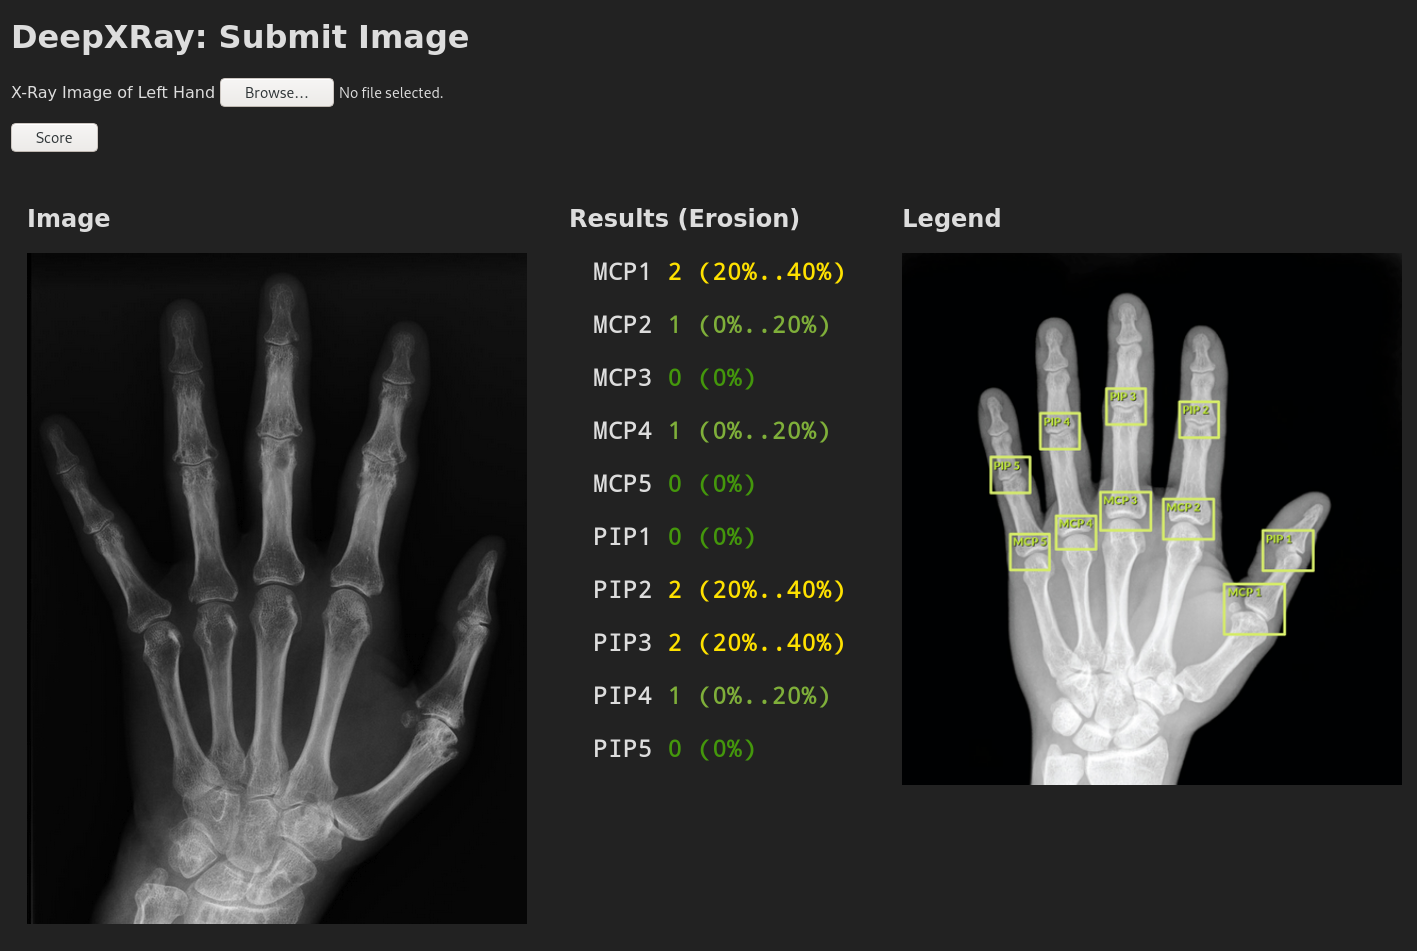
\includegraphics[width=\linewidth]{pics/web-ui-demo.png}
    \caption{Die Web-Oberfläche, auf der links das verarbeitete Röntgenbild (\textit{Case courtesy of Assoc Prof Frank Gaillard, Radiopaedia.org, rID: 3031}), in der Mitte die Scoring-Ergebnisse und rechts eine Legende mit beschrifteten Gelenken zu sehen sind. Die Schädigungen der Gelenke bewegen sich im tiefen bis mittleren Bereich.}
    \label{fig:webgui}
\end{figure}

\clearpage
